

\setcounter{chapter}{6}

\chapter{Convolutional Neural Networks - Supplementary Notes}

Unofficial notes by Shaunticlair Ruiz


\section{Introduction}

    \subsection{Fully Connected Networks}

        Up to this point, we've focus on "fully connected" neural networks. 
        
        They're called "fully connected" because between two layer, every single unit in one layer can affect every single unit in the next layer, via some weight.\\
        
        \begin{definition}
            A \vocab{fully connected} layer is ones where every number in the \purp{input} is connected (by a weight) to every element in the \purp{output}. 
        \end{definition}
        
        For example, unit $a$ in the first layer is multiplied by $w_{a,b}$ to affect unit $b$ in the second layer, for every single $a^{th}$ input and $b^{th}$ output.
        
        In this case, we have as many connections as possible, so we use this when we don't know enough about our problem: we let the machine decide how to handle it.
        
        But, this isn't always the most effective way to structure our algorithm. To show why this is, we'll introduce a particular type of problem: image processing. 
    
    \subsection{A different type of problem}
    
        For example, we might think of face recognition, or the vision used by self-driving cars.
        
        We'll simplify for now by assuming we're working with black and white images. Let's start by thinking about how we'd put our image into our fully connected network.
        
        Our image has the dimensions $(r \cross k)$: $r$ pixels wide, $k$ pixels tall.
        
        So, we list our pixels out in a single line of $rk$ inputs: this process of turning a 2d input into a 1d input is called "flattening".\\
        
        \begin{definition}
            \vocab{Flattening}: Taking an entire \purp{matrix} of inputs, and turning them into a single \purp{vector}, by listing all the numbers in a single line.
        \end{definition}
    
    \subsection{What's wrong?}
    
        Here, we present two issues:
        
            \begin{itemize}
                \item First: our computer has no concept of pixels being near or far from each other, except in the same row. 
                
                    If two pixels were on top of each other, the computer loses that information when you line up the pixels. Are they diagonal? How close are they?
                
                    Arguably, the computer could figure out the shape eventually. But, that's time wasted, and could create a less robust solution.
                    
                    We want our computer to know how the 2d \redd{space} in our image works, so it's "spatial". 
                    
                    Specifically, we want to know what pixels are nearby- which ones are \redd{local}? We're talking about "locality". 
                    
                    The combination of these two is\\
                
                    \begin{definition}
                    
                        \vocab{Spatial locality} asks: Which pixels are \purp{near} each other in \purp{space}, and how? 
                    \end{definition}
                    
                    How big a block of pixels do we need to know in order to find, say, a cat? 
                    
                    These kinds of questions fall under "spatial locality".
            
                \item Second: imagine if your computer is looking for something: maybe a cat, for example. If you move the cat within the image, it should still recognize it, right?
                
                    The problem is, in a fully connected network, it doesn't! 
                    
                    If it finds the cat in the top-left of one image, that includes different inputs than if it finds the cat in the bottom right of the image.
                    
                    We want our computer to know that these two are the same: meaning nothing \textit{changes}. Something that doesn't change is "invariant".
                    
                    The shift we just described (sliding the cat around the image) is called a "translation.
                    
                    So, the combination here is\\
                    
                    \begin{definition}
                    
                        \vocab{Translation Invariance:} The pattern you're looking for is the \purp{same}, no matter \purp{where} in the image you look for it. 
                    \end{definition}
                    
                    We'll come up with a strategy to handle both of these problems.
                
                
        
        
    \end{itemize}











\pagebreak
\section{Filters - Introduced}
    
    \subsection{The pieces of our solution}
    
        Let's figure out how to solve those two problems at once - we want to do a calculation that doesn't depend on location, for example.
        
        So, we'll make a smaller calculation at multiple different positions.
        
        And we want this calculation that gives an idea of "locality": which pixels are near each other.
        
        The solution is to do a calculation over a small region of an image (local) and repeat it all over!
        
        That might not be entirely clear right now, but we'll get into the details.
    
    \subsection{Looking for patterns}
    
        We call this calculation a filter. Here's how it works:
        
        Let's say we're looking for some pattern; we could say we're "filtering for" this pattern.
        
        So, we'll take each section of the image, and look for this matching patterns.
        
        We need an idea of how similar these patterns are. We're not sure how to do that... let's try to do a 1-D example, for inspiration.
        
        This isn't an entirely useless example, either - when you want to do sound processing, you'll have 1D data, just like this!
    
    \subsection{The 1D case}
    
        We have some string of numbers that's length $r$, and a pattern we're looking for, length $n$. So, we'll look at every length-$n$ segment of our input.
        
        Which means, we'll be comparing two length-$n$ lists of numbers, i.e. vectors.
        
        This might be registering something familiar, or maybe it isn't - but, it turns out, you can measure how similar two vectors are using the dot product!
        
        The dot-product, as we've seen in cases like linear classification ($\theta^T x$, for example), has two interesting ideas we care about.
    
    \subsection{Dot Products}
    
        To make explaining easier, let's assume $i$ represents the dimension we're focused on, and $v$ and $w$ are our two vectors.
        
        \begin{itemize}
            \item The dot product can be calculated by multiplying together the each dimension of each vector ($v_iw_i$, $v_jw_j$, so on) and adding all of those together
            \item This operation can sort of measure how "similar" these vectors are
        \end{itemize}
        
        The "similarity" idea makes the most sense if you imagine we have a binary input with 1's and -1's: 
        
        \begin{itemize}
            \item if you multiply 1 by 1, you get 1, and the two vectors are the same in that dimensions.
            \item if you multiply -1 by 1, you get -1: the two vectors are opposite (most dissimilar!) in that dimension.
            \item if you multiply -1 by -1, you get 1, the two dimensions are more similar again.
        \end{itemize}
        
        So, if our dot product is more positive, then our vectors are more similar. The same general logic works (sort of) for non-binary outputs.
    
    \subsection{Finally, 1D filtering}
    
        Back to the example we're working on: one of these two vectors is the pattern we're looking for. 
        
        So, this dot product is a good measure of how similar this piece is to that pattern! That's exactly what we're looking for - a pattern detector.
        
        So, for every substring inside this input, we'll calculate this measure of similarity - the resulting new vector is our output.
        
        If all of the number are too positive or negative, maybe we'll add a bias, where we either subtract from or add to our dot product. 
        
        This procedure is called \redd{convolution}.\\
        
        \begin{definition}
            \vocab{Convolution}: the process of looking for a \purp{pattern} in an image (or any signal) by \purp{sliding} it over the input, and repeatedly doing a \purp{dot product}-like calculation.
        \end{definition}
    
    \subsection{A comment about our output}
    
        Notice that, in this case, our output smaller than our input: because our filter can only go as far right as our vector allows, our length has shrunk by $n-1$.
        
        Why that number? Well, if we have a length-1 filter, we're all good. If we have a length-2 filter, our filter can start on every input, except for the very last one, so it has shrunk by 1.
        
        So on and so forth: every element after the first of our filter "blocks" the start of our filter from using that element.
        
        How do we deal with that? Well...
        
    \subsection{Padding}
    
        One very common solution is to do something called "padding".
        
        The idea is: our output shrank because our filter is limited by how long it is - it can't shift past the matrix; it has nothing to multiply with.
        
        So, what if we... let it stick out the side?
        
        How do we do this? Well, the reason we can't shift the filter outside the matrix is because we are missing some values. 
        
        So... we'll just add some extra values to the edge of the vector.
        
        We can pad with whatever values we want, but most often, you pad with 0's. You can also adjust how many 0's you pad with, depending on how big you want your output to be.\\
        
        \begin{definition}
            \vocab{Padding} is when you add filler values (usually 0's)to the \purp{edge} of your input so your filter can scan over the whole input, without being stopped by the edge.
        \end{definition}
        
        
    
    \subsection{A specific example - a length-2 filter}
    
        Here, we introduce a concrete example. We have a filter of size two, and take a 1-dimensional, binary "image" to start off with.
        
        
        First, our first filter is $F_1 = (-1, +1)$.  
        
        This filter looks for a very simple pattern: a smaller element on the left, and a larger element on the right. You could think of this as the numbers "increasing" from left to right.
        
        Then given the first image below, we can "convolve" it with filter $F_1$, like so.
        
        %%SHOULD PROBABLY FIX TO PUT IT IN THE LEFTMOST SLOT
        
        
        
        \begin{tikzpicture}[x=0.7cm, y=0.7cm, step=0.7cm]
          %LPK: to make this work with includeonly, due to a bug in tex, we
          %have to define this counter in the preamble
          %\newcounter{col}
          \begin{scope}
            \draw (0, 0) grid (10, 1);
            \setcounter{col}{1}
            \foreach \p in {0,0,1,1,1,0,1,0,0,0} {
              \edef\x{\value{col} - 0.5}
              \node[anchor=center] at (\x, 0.5) {\p};
              \stepcounter{col}
            }
            \node[left] at (0,0.5) {Image:};
            \draw (0, -2) grid (2, -1);
            \node[left] at (0, -1.5) {$F_1$:};
            \node[anchor=center] (f11) at (0.5, -1.5) {-1};
            \node[anchor=center] (f12) at (1.5, -1.5) {+1};
        
            \coordinate (x1) at (0.5, 0);
            \coordinate (x2) at (1.5, 0);
            \draw[->] (x1) -- ++(0,-1);
            \draw[->] (x2) -- ++(0,-1);
            \draw[->] (x1)++(0,-2) -- ++(1,-1);
            \draw[->] (x2)++(0,-2) -- ++(0,-1);
          \end{scope}
          
          \begin{scope}[yshift=-2.8cm]
            \draw (0, 0) grid (10, 1);
            \setcounter{col}{1}
            \foreach \p in {,0,1,0,0,-1,1,-1,0,0} {
              \edef\x{\value{col} - 0.5}
              \node[anchor=center] at (\x, 0.5) {\p};
              \stepcounter{col}
            }
            \node[left] at (0,0.5) {After convolution (w/ $F_1$):};
            \draw[very thick] (2, 0) grid (3, 1);
            \draw[very thick] (6, 0) grid (7, 1);
          \end{scope}
        \end{tikzpicture}
        
        
        As shown above, we do this operation for every pair of numbers in the image, to get the post-convolution result.
        
        Notice that this calculation detects exactly what we're looking for - any time we have an increasing sequence of two numbers, we get a 1 in the output!
        
        
        
        
        
    \subsection{Another example - a length-3 filter }
    
    Let's try another example: to show that we can apply convolutions one-after-another, we'll use the previous output as our new input - our new image.
    
    This filter will be length 3: we'll use $F_1 = (-1, +1, -1)$
    
    This pattern looks like a point greater than those around it - you might think of it as a local maximum.
    
    We'll pad one zero on the left (not shown below) to make our vector shrink by only 1, instead of 2.    
    
    So, we'll see how this filter does.
          
        \begin{tikzpicture}[x=0.7cm, y=0.7cm, step=0.7cm]
          
          \begin{scope}[yshift=-2.8cm]
            \draw (0, 0) grid (10, 1);
            \setcounter{col}{1}
            \foreach \p in {,0,1,0,0,-1,1,-1,0,0} {
              \edef\x{\value{col} - 0.5}
              \node[anchor=center] at (\x, 0.5) {\p};
              \stepcounter{col}
            }
            \node[left] at (0,0.5) {After convolution (w/ $F_1$):};
            \draw[very thick] (2, 0) grid (3, 1);
            \draw[very thick] (6, 0) grid (7, 1);
          \end{scope}
          
          \begin{scope}[yshift=-6.5cm]
            \draw (0, 0) grid (10, 1);
            \setcounter{col}{1}
            \foreach \p in {,-1,0,-1,0,-2,1,-1,0,} {
              \edef\x{\value{col} - 0.5}
              \node[anchor=center] at (\x, 0.5) {\p};
              \stepcounter{col}
            }
            \node[left] at (0,0.5) {After convolution (w/ $F_2$):};
            \draw (0, 2) grid (3, 3);
            \node[left] at (0, 2.5) {$F_2$};
            \draw[very thick] (6, 0) grid (7, 1);
            \node[anchor=center] at (0.5, 2.5) {-1};
            \node[anchor=center] at (1.5, 2.5) {+1};
            \node[anchor=center] at (2.5, 2.5) {-1};
        
            \coordinate (x1) at (0.5, 4);
            \coordinate (x2) at (1.5, 4);
            \coordinate (x3) at (2.5, 4);
            \draw[->] (x1)++(0,-0.5) -- ++(0,-0.5);
            \draw[->] (x2)++(0,-0.5) -- ++(0,-0.5);
            \draw[->] (x3)++(0,-0.5) -- ++(0,-0.5);
            \draw[->] (x1)++(0,-2) -- ++(1,-1);
            \draw[->] (x2)++(0,-2) -- ++(0,-1);
            \draw[->] (x3)++(0,-2) -- ++(-1,-1);
          \end{scope}
        \end{tikzpicture}
        
        And again, it works! It only gives a positive result on the sequence $(-1, +1, -1)$, where we have a local maximum. 
        
        It also gives an especially negative result at a local minimum: $(0, -1, +1)$.
                
                
        
        
        
        
        
    
\section{Filters - In higher dimensions}
    
    So, how do we extrapolate this to higher dimensions?
    
    \subsection{Multiplication in 2D}
    
        Surprisingly, the answer is pretty simple: we just do the same operation as before, but without the perspective of vectors.
        
        Before, we did the dot product for each sub-segment. This means multiplying the components "element-wise" (multiply $i^{th}$ dimension of each vector together), and adding together those results.
        
        Now, we do the exact same: our filter is 2D, so we take every continuous 2D frame of our input, and multiply, element-by-element.
        
        The same logic as before applies: if two elements are similar, we get a larger result. If they are more different, we'll get a smaller result.
    
    \subsection{Dot products, but... bigger?}
    
        Here's one way to think about this that might be helpful, might be confusing. 
        
        Break your matrix up into rows. For each of the rows, you're multiplying element-wise - like a dot product.
        
        So, you're taking a dot product for each row, which gives the similarity for those rows. 
        
        Then you add up all these dot products ("similarities") to measure the total similarity between two matrices.
        
        In a way, because we're still multiplying and adding, you might intuitively think about this as a "bigger" dot product.
        
    %%Come up with some visual examples maybe...
    
    \subsection{Comments - Evolution}
    
        As a fun fact, these kinds of 2D filters appear in the visual part of mammal brains - including yours! 
        
        This seems to show that this way of thinking about visual information is similar to how evolution settled on it - and so it probably does a pretty good job.
        






\section{Filter Banks Pt. 1}

    \subsection{More Filters!}
    
        One filter can encode lots of information, but different filters have different data: one might look for edges, maybe another can find circles, maybe a more complicated one can find a face!
        
        What if we want to have different kinds of information, at the same time? What if we want to be able to combine these pieces of information?
        
        You might think "well, I could use multiple filters", but, how do we do that? If we have multiple filters one after another, the first one may have removed information the later ones need.
        
        So, instead, what if we use multiple filters at the same time ("in parallel") - we run each filter over the original image, and save each result?
        
        Each of these calculations creates a new matrix output, which we store separately. We end up with a bunch of matrices as our output. Each of these matrices is called a \redd{channel}.\\
        
        \begin{definition}
            \vocab{Channel}: the result of using(convolving) \purp{one filter} on an \purp{image}. If multiple filters are used, we can end up with many channels.
        \end{definition}
        
        
        
        
        
        
        
        
        
        
        
        
        
\section{How to store matrices - Tensors}

    \subsection{Our goal}
    
        Now that we have all this data to store, we need to be careful how we work with it - this is a lot to keep track of, after all.
        
        In order to do that, we'll introduce what's called a "tensor".
        
    \subsection{Building Up}
    
        Consider the following review of what we know so far.
        
        \begin{itemize}
            \item If we only have one number, we store that as a \textbf{scalar}.
            
                This scalar can be thought of like a single point - since there's no axis along which we can move, sometimes this is called "0-dimensional".
            
            \item If we have a sequence of numbers, we store that as a \textbf{vector}.
            
                You can do this by stacking scalars on top of each other in a line.
                
                You can also think of this as a 1D object, where the "dimension" is the index we can move along to get different scalars. 
                
                In a way, we have a "line" of numbers, at least visually.
            
            \item If you have several sequences of numbers, you can store that as a \textbf{matrix}.
            
                You can do this by stacking vectors next to each other. If you break your matrix up into rows or columns, you get a bunch of vectors!
                
                This is a 2D object: you can move along the rows, or the columns: each of these is a dimension. 
                
                We have a grid of numbers, or maybe you can imagine it as a square or "plane".
            
            \item What if we want to stack several matrices on each other?
            
                This would create a sort of 3D object, where we have rows, columns, and height.
                
                Visually, you might imagine the 1d case as a line of numbers, the 2d case as a square of numbers. 
                
                Now, we have what you could think of as a "cube" of numbers.
                
                This cube of numbers, this 3D object, is what we call a \textbf{tensor}.
        \end{itemize}
        
        \begin{definition}
            A \vocab{tensor} is the more "generalized" version of a matrix: it's just a \purp{"box"} of numbers in some \purp{dimension}. In our case, our \vocab{tensor} is \purp{cube} (or cuboid) of numbers.
        \end{definition}
        
         
        
        As you see in the definition above, a tensor is technically any version of this kind of object, in any dimension. A scalar, vector, and matrix are all tensors.
        
        But, for our purposes, we only care about what is called a \redd{3-tensor}, or a 3D box of numbers. The one that looks like a \purp{cube}.
        
    \subsection{An important warning: dimensions}
    
        Before we continue, we should make a quick warning about dimensions.
        
        You might have noticed that the way we are using the word "dimension" here is different from how we have used it in other parts of the course.
        
        For example, if you have a vector that has 3 elements, you could call that a "3D vector", because you can imagine it as an arrow in 3D space.
        
        But above we said vectors were "1D" objects. What gives?
        
        This is because, unfortunately, there are different ways you can talk about "dimensions".
        
        All have some different mathematical reason behind them, where in some way, they are related, \textbf{but these definitions are different and you should be careful.}
        
        Let's get into that.
        
    \subsection{Dimensions, Clarified}
    
        We'll break this down. Dimensions are about asking the question, "how many separate ways can I change what I'm looking at?"
        
        For example, we live in 3D space because we can vary our position in the $x$, $y$, and $z$ directions.
        
        A paper is 2D because there are only two separate ways to move on the paper.
        
        Based on this, we can think of two definitions for dimensions:
        
        \begin{itemize}
            \item Version 1: If we drew our vector in space, how many ways can we vary the direction it points in?
            
            Or, in other words, how many \textit{dimensions} of space are we thinking of when we draw our vector?
            
            This definition focused on vectors, and each number in that vector as a unique dimension. 
            
            In this perspective, we imagine that we can vary each scalar in our vector to create a different vector, and we have $n$ scalars that we can vary.
            
            To summarize:
            
            \begin{itemize}
                \item A scalar is a 1D vector.
                
                \item A vector with 2 numbers is 2D by this definition. 
                
                \item A ($4 \cross 4$) matrix (4 vectors, each in 4D), is 4D.
            \end{itemize}
            
            
            \begin{definition}
                One way to define \vocab{dimensions} is to ask how many different \purp{numbers} (scalars) we have in a \purp{vector}.
            \end{definition}
            
            
            \item Version 2: How many axes of numbers do we have to work with?
            
            This definition is more abstract, and talks about the dimension of what we're storing our numbers in. 
            
            In this perspective, we imagine that we can vary the index on each axis (row, column, height, etc.) to find a different scalar, and we have $k$ axes we can vary.
            
            To summarize:
            
            \begin{itemize}
                \item A scalar is a 0D object.
            
                \item A vector with 2 numbers is 1D by this definition. 
                
                \item A ($4 \cross 4$) matrix (4 vectors, each in 4D), is 2D.
            \end{itemize}
            
            \begin{definition}
                Another way to define \vocab{dimensions} is to ask how many \purp{axes} our \purp{box} of numbers, or \purp{tensor}, has.
            \end{definition}
            
        \end{itemize}
        
        Now that we've clarified the difference, back to tensors.
        
        
    \subsection{Back on track: What's a tensor?}
    
        Using what we've carefully built up, we have everything we need to understand the basics of tensors:
        
        A tensor is, more or less, a bunch of matrices of the same shape stacked on top of each other. 
        
        You can visualize it as a \redd{cube of numbers}.
        
        Not too bad, right?
        
    \subsection{Tensor Math (Optional)}
    
        We went through all this work to carefully build understanding because tensors are not easy, but they are very, very important. 
    
        Unfortunately, just like how matrix multiplication, algebra, and calculus have their own special operations and rules, so too, do tensors.
        
        However, simply put: tensor multiplication and calculus are really hard, so we're not going to do it. We'll let the computer handle it.
        
        The rules involved are incredibly general and very, very powerful.
        
        Physicists, computer scientists, mathematicians, and other smart people solving hard problems have to grapple with the details for years, sometimes, to understand everything they need.
        
        We do not have that time. So, we'll leave those details to the computer.
        
    \subsection{What about higher dimensions? (Optional)}
    
        One little plot twist: what if we need something even bigger than a tensor?
        
        What if we need to stack multiple tensors, for an even more complicated problem?
        
        Well, thankfully, tensors actually include things higher than 3 dimensions!
        
        If you have a "4D cube of numbers", that still follows the rules of tensors.
        
        Tensor math can be applied for any higher dimensions. So, if we were to ever need it, our computer knows how to handle it.
        
        
        
        
        
        
        
        
        
        
        
\section{Filter Banks Pt. 2}

    \subsection{Review}

        Now that we know what a tensor is, let's pick back up where we left off:
        
        We wanted to convolve multiple different filters with our image at the same time ("in parallel"). We call this collection of filters a "filter bank".\\
        
        \begin{definition}
            A \vocab{filter bank} is a collection of \purp{filters} used on the \purp{same image}.
        \end{definition}
        
        (Side comment: notice you can store this filter bank as a tensor too! Since each filter is a matrix, and you can just stack them).
    
    \subsection{Using filter banks}
    
        The output after applying all these filters is a tensor: each filter outputs to one "channel", which is what we call the third dimension of our tensor (row, column, channel)
        
        
        
        \begin{tikzpicture}[scale=0.6]
          \begin{scope}
            \draw[black,very thick] (0,0) rectangle (4,4);%marking borders
            \node[anchor=center] at (2,2) {Image};
          \end{scope}
        
          \coordinate (x) at (4.4, 2.5);
          \foreach \yoff in {-1.5,-.5,.5,1.5} {
            \draw[->,thick] (x) -- ++(2,\yoff);
          }
            
          \begin{scope}[xshift=8cm]
            \foreach \shift/\c in {10.5mm/blue,3.5mm/red,-3.5mm/green,-10.5mm/purple} {
              \begin{scope}[xshift=\shift, yshift=\shift]
                \fill[white,fill opacity=0.9] (0,0) rectangle (4,4);
                \draw[step=4mm, color=\c] (0,0) grid (4,4); %defining grids
                \draw[black,very thick] (0,0) rectangle (4,4);%marking borders
              \end{scope}
            }
            \draw [decorate,decoration={brace,mirror,amplitude=10pt}]
              (2.7,-1.4) -- node (layers) {} (5.5,1);
            \coordinate (r) at (8.2, 1);
            \draw[->,thick] ($(layers)+(1,-0.2)$) -- (r);
          \end{scope}
        
          \begin{scope}[xshift=18cm,yshift=0.75cm]
            \foreach \shift/\c in {10mm/gray,-0mm/gray,-10mm/black} {
              \begin{scope}[xshift=\shift, yshift=\shift]
                \fill[white,fill opacity=0.9] (0,0) rectangle (2,2);
                \draw[step=4mm, color=\c] (0,0) grid (2,2); %defining grids
                \draw[black,very thick] (0,0) rectangle (2,2);%marking borders
              \end{scope}
            }
          \end{scope}
        \end{tikzpicture}
        
        This diagram loosely shows the process: the first object on the left is our image. 
        
        The many arrows represents that the image is applied to each of the filters in multi-color filter bank. Finally, each of those outputs is combined into the tensor on the right.
        
        If we apply $k$ filters, we will end up with $k$ channels: one for each filter.
        
        So, if a single filter resulted in a $(r \cross r)$-sized matrix, then the filter bank results in a $(r \cross r \cross k)$ tensor.
    
    \subsection{An example: Using a Filter Bank}

        Let's show an example of 2d filtering, with a filter bank.
        
        Our filter bank has two filters, $f_1$ and $f_2$. So in this case, $k=2$.
        
        Each filter is $(3 \cross 3)$ in size. So we preserve the size in our output, we'll add 1 layer of 0-padding all the way around our input matrix (not shown).
        
        As mentioned before, each filter will be convolved with the input image, "looking" for the pattern they represent.
        
        In this case, we see that $f_1$ seems to be looking for a vertical line, and $f_2$ is looking for a horizontal line; both 3 pixels long.
        
        Our input image is $(n \cross n)$, so our output of the first step will be an $(n \cross n \cross 2)$ tensor.
        
        \begin{tikzpicture}[scale=0.4]
          \begin{scope}
            \foreach \x/\y in {0/0,0/1,0/2,2/1,2/2,2/3,3/1,3/3,4/1,4/2,4/3,
              3/5,4/5,5/5} {
              \fill[black] ($(\x,\y)$)
                rectangle ($(\x,\y)+(1,1)$);
            }
            \draw[black,thick] (0,0) grid (6,6);
            \draw[black,very thick] (0,0) rectangle (6,6);
            \draw[->,thick] (6.5,4.5) -- (13.5, 7.5);
            \draw[->,thick] (6.5,1.5) -- (13.5, -1.5);
            \begin{scope}[xshift=8.2cm,yshift=7.2cm]
              \foreach \x/\y in {0/1,1/1,2/1} {
                \fill[black] ($(\x,\y)$)
                  rectangle ($(\x,\y)+(1,1)$);
              }
              \draw[black,thick] (0,0) grid (3,3);
              \draw[black,very thick] (0,0) rectangle (3,3);
              \node[left] at (0,1.5) {$f_2$};
            \end{scope}
            \begin{scope}[xshift=8.2cm,yshift=-4.2cm]
              \foreach \x/\y in {1/0,1/1,1/2} {
                \fill[black] ($(\x,\y)$)
                  rectangle ($(\x,\y)+(1,1)$);
              }
              \draw[black,thick] (0,0) grid (3,3);
              \draw[black,very thick] (0,0) rectangle (3,3);
              \node[left] at (0,1.5) {$f_1$};
            \end{scope}
          \end{scope}
          \begin{scope}[xshift=14cm, yshift=6cm]
            \foreach \x/\y in {3/1,3/3,4/5} {
              \fill[black] ($(\x,\y)$)
                rectangle ($(\x,\y)+(1,1)$);
            }
            \draw[black,thick] (0,0) grid (6,6);
            \draw[black,very thick] (0,0) rectangle (6,6);
          \end{scope}
          \begin{scope}[xshift=14cm, yshift=-6cm]
            \foreach \x/\y in {0/1,2/2,4/2} {
              \fill[black] ($(\x,\y)$)
                rectangle ($(\x,\y)+(1,1)$);
            }
            \draw[black,thick] (0,0) grid (6,6);
            \draw[black,very thick] (0,0) rectangle (6,6);

          \end{scope}


        \end{tikzpicture}
        
        Notice that the top output puts three dots where it finds horizontal lines( you can match them up visually!)
        
        The bottom output puts three dots where it finds vertical lines. So, it seems to be working!
        
\section{Tensor Filters}

    \subsection{What now?}

        Now we have used multiple filters, and we got a tensor... great! 
        
        But... what on earth do we do with a tensor?
        
    \subsection{Motivation}
    
        So, the whole reason we used multiple filters, was so we could look for multiple patterns at the same time.
        
        Often, the goal of your trained machine is to recognize certain shapes.
        
        It may be easier to look for smaller, simpler shapes first, and then combine those results to look for bigger shapes; and so on.

        For example: imagine you're looking in an image for a child's depiction of a house. 
        
        You might look for the signature rectangle on the bottom, and a triangle "roof" on top. These are two distinct features you can find with different filters.
        
        So, using our previous steps, we have a filter that finds squares, and one that finds triangles.
        
        But what about combining them?
        
    \subsection{Filters, again!}
    
        The solution is to use another filter!
        
        But this time, we need to go up a dimension again.
        
        We went from 1D filters to 2D filters because we wanted to look for 2D patterns, and we did this by multiplying element-wise as we moved across the grid.
        
        Now, we have a 3D tensor we're analyzing. 
        
        In this case, we want to find a point on one layer (representing the roof), closer to the top of the image than a point in the next layer (representing the "body" of the house)
        
        So, if this is the pattern we're looking for, we could replicate this pattern in a new filter! We'll create a tensor that represents this pattern, and again, slide this pattern around the image.
        
        For simplicity's sake, we'll assume this tensor has the same number of channels as the input, so we only have to slide it around the image, and not through the different channels (doesn't that sound complicated...)
        
        Thus, we have invented the "tensor filter". All the same math from before (multiplying element-wise, sliding around the image, maybe padding...) is the same.
        
    \subsection{An example}
    
        We'll take the output from our earlier example and run a tensor filter over it.
        
        Let's say the output we're looking for a "circle", or really, a ($3 \cross 3)$ square with a hole in the center.
        
        This is gotten by having two vertical lines on the sides, and two horizontal lines on top and bottom of the section of the image.
        
        So, we'll create a filter so that's exactly what we're looking for!
        
        One channel will look for the two horizontal lines, the other will look for the two vertical lines.
        
        Remember that below, the top image gave us horizontal lines, and the bottom image gave us vertical lines.
        


        \begin{tikzpicture}[scale=0.4]
        
        
        
          \begin{scope}[xshift=14cm, yshift=6cm]
            \foreach \x/\y in {3/1,3/3,4/5} {
              \fill[black] ($(\x,\y)$)
                rectangle ($(\x,\y)+(1,1)$);
            }
            \draw[black,thick] (0,0) grid (6,6);
            \draw[black,very thick] (0,0) rectangle (6,6);
            \draw[->,thick] (6.5,1.5) -- (13.5, -1.5);
          \end{scope}
          \begin{scope}[xshift=14cm, yshift=-6cm]
            \foreach \x/\y in {0/1,2/2,4/2} {
              \fill[black] ($(\x,\y)$)
                rectangle ($(\x,\y)+(1,1)$);
            }
            \draw[black,thick] (0,0) grid (6,6);
            \draw[black,very thick] (0,0) rectangle (6,6);
            \draw[->,thick] (6.5,4.5) -- (13.5, 7.5);
          \end{scope}
          \begin{scope}[xshift=22cm,yshift=1.5cm]
            \foreach \x/\y in {1/0,1/2} {
              \fill[black] ($(\x,\y)$)
                rectangle ($(\x,\y)+(1,1)$);
            }
            \draw[black,thick] (0,0) grid (3,3);
            \draw[black,very thick] (0,0) rectangle (3,3);
        
            \begin{scope}[xshift=-0.35cm,yshift=-0.35cm]
              \fill[white,fill opacity=0.8] (0,0) rectangle (3,3);
              \foreach \x/\y in {0/1,2/1} {
                \fill[black] ($(\x,\y)$)
                  rectangle ($(\x,\y)+(1,1)$);
              }
              \draw[black] (0,0) grid (3,3);
              \draw[black,very thick] (0,0) rectangle (3,3);
              \node[left] at (0.4,1.5) {\begin{tabular}{c}tensor\\
                                                        filter\end{tabular}};
            \end{scope}
          \end{scope}
          \begin{scope}[xshift=28cm]
            \fill[black] (3,2) rectangle (4,3);
            \draw[black,thick] (0,0) grid (6,6);
            \draw[black,very thick] (0,0) rectangle (6,6);
          \end{scope}
        \end{tikzpicture}
        
        Like magic, we get exactly what we're looking for! Notice that it has a dot in exactly one place. If we go back to the original...
        
        \begin{tikzpicture}[scale=0.4]
          \begin{scope}
            \foreach \x/\y in {0/0,0/1,0/2,2/1,2/2,2/3,3/1,3/3,4/1,4/2,4/3,
              3/5,4/5,5/5} {
              \fill[black] ($(\x,\y)$)
                rectangle ($(\x,\y)+(1,1)$);
            }
            \draw[black,thick] (0,0) grid (6,6);
            \draw[black,very thick] (0,0) rectangle (6,6);

          \end{scope}
        \end{tikzpicture}
        
        We have our dot right in the center of our empty square/"circle"! We can see that the process works.
        
        Here's what the whole thing looks like when we put it together:
        
        \begin{tikzpicture}[scale=0.4]
                
          \begin{scope}
            \foreach \x/\y in {0/0,0/1,0/2,2/1,2/2,2/3,3/1,3/3,4/1,4/2,4/3,
              3/5,4/5,5/5} {
              \fill[black] ($(\x,\y)$)
                rectangle ($(\x,\y)+(1,1)$);
            }
            \draw[black,thick] (0,0) grid (6,6);
            \draw[black,very thick] (0,0) rectangle (6,6);
            \draw[->,thick] (6.5,4.5) -- (13.5, 7.5);
            \draw[->,thick] (6.5,1.5) -- (13.5, -1.5);
            \begin{scope}[xshift=8.2cm,yshift=7.2cm]
              \foreach \x/\y in {0/1,1/1,2/1} {
                \fill[black] ($(\x,\y)$)
                  rectangle ($(\x,\y)+(1,1)$);
              }
              \draw[black,thick] (0,0) grid (3,3);
              \draw[black,very thick] (0,0) rectangle (3,3);
              \node[left] at (0,1.5) {$f_2$};
            \end{scope}
            \begin{scope}[xshift=8.2cm,yshift=-4.2cm]
              \foreach \x/\y in {1/0,1/1,1/2} {
                \fill[black] ($(\x,\y)$)
                  rectangle ($(\x,\y)+(1,1)$);
              }
              \draw[black,thick] (0,0) grid (3,3);
              \draw[black,very thick] (0,0) rectangle (3,3);
              \node[left] at (0,1.5) {$f_1$};
            \end{scope}
          \end{scope}
          \begin{scope}[xshift=14cm, yshift=6cm]
            \foreach \x/\y in {3/1,3/3,4/5} {
              \fill[black] ($(\x,\y)$)
                rectangle ($(\x,\y)+(1,1)$);
            }
            \draw[black,thick] (0,0) grid (6,6);
            \draw[black,very thick] (0,0) rectangle (6,6);
          \end{scope}
          \begin{scope}[xshift=14cm, yshift=-6cm]
            \foreach \x/\y in {0/1,2/2,4/2} {
              \fill[black] ($(\x,\y)$)
                rectangle ($(\x,\y)+(1,1)$);
            }
            \draw[black,thick] (0,0) grid (6,6);
            \draw[black,very thick] (0,0) rectangle (6,6);

          \end{scope}
        
          \begin{scope}[xshift=14cm, yshift=6cm]
            \foreach \x/\y in {3/1,3/3,4/5} {
              \fill[black] ($(\x,\y)$)
                rectangle ($(\x,\y)+(1,1)$);
            }
            \draw[black,thick] (0,0) grid (6,6);
            \draw[black,very thick] (0,0) rectangle (6,6);
            \draw[->,thick] (6.5,1.5) -- (13.5, -1.5);
          \end{scope}
          \begin{scope}[xshift=14cm, yshift=-6cm]
            \foreach \x/\y in {0/1,2/2,4/2} {
              \fill[black] ($(\x,\y)$)
                rectangle ($(\x,\y)+(1,1)$);
            }
            \draw[black,thick] (0,0) grid (6,6);
            \draw[black,very thick] (0,0) rectangle (6,6);
            \draw[->,thick] (6.5,4.5) -- (13.5, 7.5);
          \end{scope}
          \begin{scope}[xshift=22cm,yshift=1.5cm]
            \foreach \x/\y in {1/0,1/2} {
              \fill[black] ($(\x,\y)$)
                rectangle ($(\x,\y)+(1,1)$);
            }
            \draw[black,thick] (0,0) grid (3,3);
            \draw[black,very thick] (0,0) rectangle (3,3);
        
            \begin{scope}[xshift=-0.35cm,yshift=-0.35cm]
              \fill[white,fill opacity=0.8] (0,0) rectangle (3,3);
              \foreach \x/\y in {0/1,2/1} {
                \fill[black] ($(\x,\y)$)
                  rectangle ($(\x,\y)+(1,1)$);
              }
              \draw[black] (0,0) grid (3,3);
              \draw[black,very thick] (0,0) rectangle (3,3);
              \node[left] at (0.4,1.5) {\begin{tabular}{c}tensor\\
                                                        filter\end{tabular}};
            \end{scope}
          \end{scope}
          \begin{scope}[xshift=28cm]
            \fill[black] (3,2) rectangle (4,3);
            \draw[black,thick] (0,0) grid (6,6);
            \draw[black,very thick] (0,0) rectangle (6,6);
          \end{scope}
        \end{tikzpicture}
        
    We can see the full process of running two separate filter banks, and getting the results we're looking for.
    
    \subsection{Really small side comment: RGB color (Optional)}
    
        If your image is RGB (made up of red, green, blue), you'll need three values at every pixel: this is most easily described with a tensor!
        
        So, if you have an image that is $(n \cross n)$ in size, the RGB representation will be a tensor of the shape $(n \cross n \cross 3)$.
    
\section{Machine learning and Convolution}

    \subsection{Applying to ML: Layering}
    
        Now, we have learned how to use convolution to process information. 
        
        We can see it's good for finding patterns, so it makes some sense we'd want to add that ability to our network.
        
        So, let's try that: how do we use convolution in our neural network?
        
        Well, because our network is modular (broken up into separate pieces, or "modules", that can be thought of separately), the process isn't too painful.
        
        All we have to do is insert a new layer of convolution into our neural network. 
        
        It takes in inputs from whatever the last layer gave, and sends its output to the next layer after. 
        
        In fact, our example above shows two consecutive layers of convolution.
        
        This can be used to build larger features (circles) from smaller ones (lines).
        
    \subsection{Thinking in ML terms}
        
        Each filter bank we use will represent a single layer.
        
        If we want to think in the terms of ML, we can think of each number inside a filter as a "weight": a number used for calculation we can adjust.
        
        As we mentioned early on, we might also have one bias for our filter - making the output of our element-wise multiplication more positive, more negative, etc.
        
    \subsection{Training Filters}
    
        In the past, machine vision experts would hand-craft their filters, and experiment with them. 
        
        However, because we can think of our filters in terms of their weights, we can use gradient descent to train them!
        
        As long as we can take our derivatives, we can use gradient descent to find better filters. Our computers know how to do this.
        
        Sometimes, these filters can even tell us about the structure of the data!
        
        
    \subsection{Benefits of Convolution}
    
        This convolution has a lot of benefits. Two of those were the original motivations for trying out convolution:
        
        \begin{itemize}
            \item \textbf{Spatial Locality}: A filter tells you about what the "local" area around a pixel looks like.
            
            Thus, it can give the neural network the ability to associate that information.
            
            \item \textbf{Translation Invariance}: A filter also, by virtue of being slid around, will find the same pattern no matter where in the image it appears.
            
            This means the neural network can now more easily tell that an object in the bottom right is often the same as an image in the top left.
            
        \end{itemize}
        
        But there's one more surprising benefit: efficiency.
    
    \subsection{Efficiency of Convolution: Fewer Weights}
        
        The interesting detail: a filter is (typically) much smaller than an image, and each pixel in the filter only has one weight. 
        
        So, rather than having many weights for every pixel in the input, we have a small number of weights for our filter.
        
        On top of that, these weights are reused multiple times during convolution, as we slide around the image.
        
        So, we have a much, much smaller number of weights to train.
        
        Because we are "sharing" weights between different calculations, we call this benefit \redd{weight sharing}.
        
        \begin{definition}
            \vocab{Weight sharing} is where the \purp{same weights} are used for \purp{multiple calculations}. Thus, the model trains \purp{faster}.
        \end{definition}
        
        For example:
        
        if we have a $(5 \cross 5)$ image, and want a $(5 \cross 5)$ output, using a fully connected layer, we would need 25 inputs, 25 outputs. 
         
        This creates $25*25$ weights, and $25*1$ biases: 650 parameters.
         
        If we have a $(3 \cross 3)$ filter, and we use length-1 padding all the way around the image, we can get the same size output.
         
        This has $3*3$ weights, and 1 bias: 10 parameters.
        
        And this efficiency grows the larger your input and output are.
        
        This does mean we have to be careful when training, though!

    \subsection{Variable definitions}
    
        Let's carefully define this with some variables. Let's say we place our filter bank on layer $l$. 
        
        Note that we'll assume the image and filter are both square (same number of rows and columns). 
        
        This isn't necessary, but makes our definition simpler.
        
        Additionally, remember that exponents in this notation only represent which layer you're referring to.
        
        Our variables:
        
        \begin{itemize}
            \item \textbf{Length} of the square \textbf{input}: $n^{l-1}$
            
            We use $l-1$ instead of $l$ because this is technically the \textbf{output} of the previous layer.
        
            \item \textbf{Number} of \textbf{filters}: $m^l$
            
            \item \textbf{Length} of each square \textbf{filter}: $k^l$
            
            \item \textbf{Padding} around the \textbf{input}: $p^l$
            
            Remember that we usually pad with the number 0.
        \end{itemize}
        
        For each filter, we also have one additional bias term. 
        
        To use this bias, we do the element-wise multiplication, add up the terms, and \textit{then} add the bias.
        
        We have one bias per filter, or $m^l$ total biases in a layer.
        
    
    \subsection{Shapes}
        
        Now, we need to find the shape of each object.
        
        If we have only \textbf{one filter}, we just end up with some squares:
        
        \begin{itemize}
            \item  Our filter: $(k^l \cross k^l)$
            \item  Our input: $(n^{l-1} \cross n^{l-1})$
        \end{itemize}

        
        What if our previous layer had filters, though?
            
        Well, if our previous layer had $m^{l-1}$ filters, then it would give the output (our new input) a third dimension of $m^{l-1}$.
        
        We mentioned before we only want to slide our filter across rows and columns, so the third dimension needs to match.
        
        Thus, we need our filter to have as many channels as these previous output: our third dimension is $m^{l-1}$.
        
        Thus, our shapes are
        
        \begin{itemize}
            \item  Our filter: $(k^l \cross k^l \cross m^{l-1})$
            \item  Our input: $(n^{l-1} \cross n^{l-1} \cross m^{l-1})$
        \end{itemize}
        
    
\section{Output dimensions}

    Let's round out some other important considerations related to size. Specifically, we'll look at things affecting the output dimensions.
    
    \subsection{Filter Size}
    
        Recall that, in the 1D case, we showed that our output (vector) dimension is decreased by $k-1$.
        
        This was because every element of the filter after the first prevented the filter from moving further to the right.
        
        We can extrapolate the same concept to multidimensional inputs: each dimension is shrunk by $k-1$.
        
        So, an $(n \cross n)$ input turns into a $( (n-k+1) \cross (n-k+1) )$ output.
        
        For the rest of the problem, we shall refer to $n$- squares to mean squares of length $n$, rather than writing out the full dimensions.
        
        So in this case, the length is
        
        \begin{equation*}
            n^{l} = n^{l-1}-k^{l}+1
        \end{equation*}
        
        
    
    \subsection{Padding}
        
        We have mentioned padding, but it's important to remember how this affects the input and output.
        
        If we add padding symmetrically all the way around the input, then we add $p$ 0's to the left of our image, and $p$ 0's to the right. 
        
        So, the dimension increases by $2p$.
        
        Thus, we can say our $n$-square has its length changed to 
        
        \begin{equation*}
            n^{l} = n^{l-1}+2p^l
        \end{equation*}
        
    \subsection{Stride}
    
        Here, we introduce a new concept: stride.
        
        When we convolve normally, we move our filter over by 1 for each step.
        
        But, we could also move over by $r$ for each step. Basically, we "skip over" several pixels each time. 
        
        A stride of 1 means we move our pixel over by one each time, same as normal.
        
        A stride of 2 means we move our pixel over by 2 each time: you "skip" every even pixel.
        
        In 1D, you would convolve with pixel 1, 3, 5...\\
        
        \begin{definition}
            \vocab{Stride}: How many \purp{pixels} you \purp{slide} over with each \purp of convolution.
        \end{definition}
        
        As you can see, we skip one pixel each time, the size of our output image becomes half the size.
        
        So we start by guessing we get a square of length $n/s$.
        
        We have to round, though: if we have a stride of 2, and 5 pixels, that would imply a length 2.5 square.
        
        But as we can see above, if we have 5 pixels, we have 3 pixels to convolve with.
        
        Rounding up has its own notation: if you want to round up $x$, you write that as $\lceil x \rceil$
        
        So, we get a square of length 
        
        \begin{equation*}
            n^{l} =\lceil n^{l-1}/s^l \rceil
        \end{equation*}
    
    \subsection{The convolution output size}
    
        We combine all three of these factors to get a single equation.
        
        \begin{itemize}
            \item Filter size: $n-k+1$
            \item Padding: $n+2p$
            \item Stride: $\lceil n/s \rceil$
        \end{itemize}
        
        We get this result (which is important, and worth saving!):
        
        \begin{equation*}
            n^{l} = \lceil ( n^{l-1} - k^l + 1 + 2p^l)/s^l \rceil
        \end{equation*}
        
        
        

\section{Max Pooling}

    \subsection{Gathering information}
    
        As we've alluded to, convolution can be used to get basic features, which we combine into larger features later.
        
        Whether lines into circles, or shapes into childlike houses, we often want to combine these patterns.
        
        However, as we gather this information, it might make sense for us to shrink the output.
        
        Why? Well, there are going to be many more small, simple patterns (like edges) in an image than large, complex ones (like a house).
        
        This is natural: if it takes many edges to make one house, there will be fewer houses than edges.
        
        So, combining our outputs into a smaller image let's us get a "bigger picture" on whatever is going on.
        
    \subsection{How to combine patterns}
    
        Our first thought might be to increase the filter size, or increase the stride size.
        
        However, these both present problems: we may not want a larger filter, and using one might focus on patterns we don't care about.
        
        Meanwhile, even though stride size makes the image smaller, you lose some information:
        
        If the pattern is between two of your stride steps, for example, you might miss it. So, greater stride doesn't collect all the information over that range.
        
        What we'll do instead is a new tool called \textbf{max pooling}.
    
    \subsection{What is max pooling?}
    
        Max pooling is a tool similar to ones we've used before, but with its own twist.
        
        It behaves like a filter: we pick a size we're looking over, do a calcuation, and then move our "window" around all over the input.
        
        Sometimes we call the area that we're currently applying our filter to (to get the maximum value) the "receptive field" or just a "field".
        
        So, we get the maximum value over our "receptive field".
        
        \begin{definition}
            \vocab{Receptive Field}: the \purp{portion} of our input we're currently \purp{applying} our \purp{filter} to.
        \end{definition}
        
        In this case, however, the calculation is different: all we do is \textbf{return the largest value over a certain range}.\\
        
        \begin{definition}
            \vocab{Max pooling} is the process of looking over our \purp{field} and returning the \purp{maximum} value over that region.
        \end{definition}
        
        
        
        For an example: consider a $(3 \cross 3)$ max pool window.
        
        We would take a 3-length square and slide it around our input image, and for every position, we put the maximum value in a new output matrix.
        
        
    \subsection{Considerations for Max Pooling}
    
        A few comments:
        
        First, notice that, since we're taking the maximum, there are no weights: the layer always operates in the same way.
        
        In fact, there is no bias, either.
        
        You can think of this kind of like a ReLU layer, which also has no weights, because it only relies on a simple function.
        
        Because of this, we might call it a "pure functional layer".
        
        Second, it has filter size, so it decreases size according to its size and stride, just like a regular filter.
        
        Finally, remember that the goal of our max pooling layer is meant to aggregate information. So, we put two restrictions:
        
        \begin{itemize}
            \item Our stride $s > 1$ , so we end up with a smaller output.
            
            Hopefully, this is how we collect our information together.
        
            \item Our filter width $k \geq s$. This is so we don't skip over some values.
            
                To understand why, consider that if we had a stride of 5, and a filter width of 1, then we would never touch a large part of our input!
                
                We could miss crucial information that way.
                
        \end{itemize}
        
        Because we're only taking the maximum over a broad area, we lose some of the precise information about where a pattern was found. 
        
        This can take away some information, but it lets our machine learn to find patterns regardless of where they are.
        
    \subsection{An example}
    
        For example, let's take a matrix of size $(64 \cross 64 \cross 3)$.
        
        We'll set our filter to size 2, with stride 2.
        
        Using our equation for the size of our output, we get
        
        \begin{equation*}
            \lceil ( 64 - 2 + 1 )/2 \rceil = \lceil ( 63 )/2 \rceil = 32
        \end{equation*}
        
        So, our output dimensions are $(32 \cross 32 \cross 3)$.
        
    \subsection{Concerns about Max Pooling}
    
        One problem with max pooling is that they don't perfectly handle "translation invariance", or, our algorithm not caring exactly where our pattern is.
        
        This is because, if your stride $s>1$, then you could shift the pattern within that stride to change the max pooling output significantly.
        
        This problem will not be elaborated further here, but here's a relevant paper (https://arxiv.org/pdf/1904.11486.pdf)




\section{Typical architecture}

    \subsection{An example of a CNN}
    
        Here, we give the form for a "typical" convolutional network:
        
        \begin{figure}[H]
            \includegraphics[width=\textwidth]{images/convolutional_neural_networks_images/Architecture.png}
            
            \caption*{The ``depth'' dimension in the layers shown as cuboids corresponds to the number of channels in the output tensor. (Figure source: https://www.mathworks.com/solutions/deep-learning/convolutional-neural-network.html)}
        \end{figure}
        
    
    \subsection{Common features of CNNs}
        
        First and foremost: a CNN is just a regular neural network, with some convolutional layers, like filters and max pooling.
        
        Here, we get into some common features:
        
        \begin{itemize}
            \item After each filter layer there is generally a ReLU layer
            \item there maybe be multiple filter/ReLU layers
            \item Max pooling is often used after filtering to shrink the output.
            \item Once the output is relatively small, we finish with a fully-connected layer
            \item We close out with our activation function. For example, we might use softmax in a classification problem.
        \end{itemize}
        
        There's very few hard rules for how exactly to design this kind of network.
        
        There are no good guidelines, either in theory or in practice, to tell us how our choice affects how well the networks does.

\section{Training our Network}

    \subsection{Can we train it?}
    
        Given the subject matter of this course, "Machine Learning", your first question might be, can we train this, and if so, how?
        
        Well, thankfully, it turns out we can!
        
        The various weights of filters and other components are (mostly) continuously differentiable, so we can return to our old friend, back-propagation.
        
        (Technically ReLU and max pooling both don't have continuous derivatives, but we can usually get away with this)
        
    \subsection{An example}
    
        We'll try a simple example, just to understand how we can do back-propagation on convolutional networks.
        
        \begin{center}
            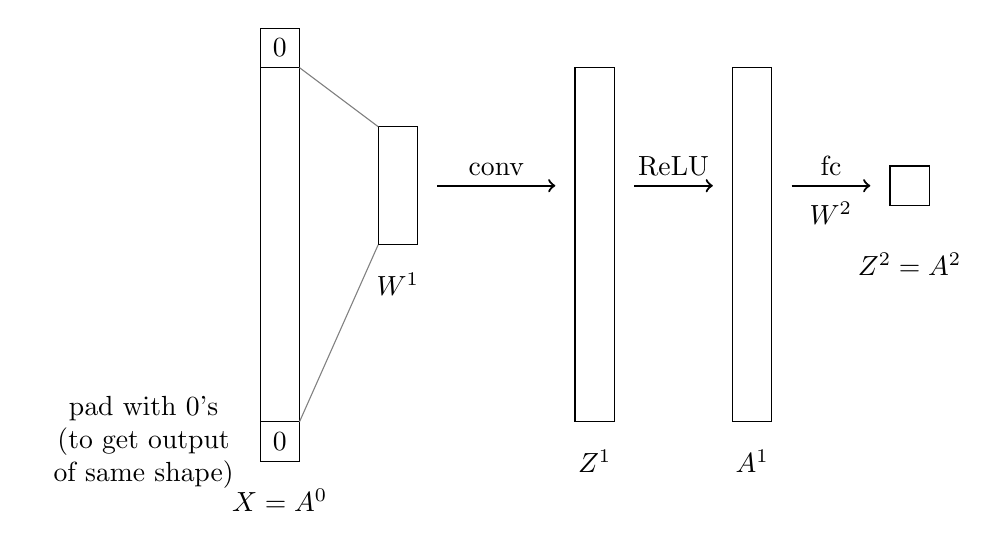
\begin{tikzpicture}[scale=0.5]
              \draw (0,0) rectangle (1,9);
              \node at (.5, -2) {$X = A^0$};
              \draw (0,-1) rectangle (1,0);
              \draw (0,9) rectangle (1,10);
              \node[anchor=center] at (0.5,-.5) {0};
              \node[anchor=center] at (0.5,9.5) {0};
              \node[left] at (0,-0.5) {\begin{tabular}{c}
                pad with 0's\\ (to get output\\ of same shape)\end{tabular}};
            
              \draw (3,4.5) rectangle (4,7.5);
              \draw[gray] (1,9) -- (3,7.5);
              \draw[gray] (1,0) -- (3,4.5);
              \node at (3.5,3.5) {$W^1$};
            
              \draw (8,0) rectangle (9,9);
              \node at (8.5,-1) {$Z^1$};
            
              \draw (12,0) rectangle (13,9);
              \node at (12.5,-1) {$A^1$};
            
              \draw (16,5.5) rectangle (17,6.5);
              \node at (16.5, 4.0) {$Z^2=A^2$};
            
              \node at (14.5,5.3) {$W^2$};
            
              \draw[->,thick] (4.5,6) -- node[above] {conv} (7.5,6);
              \draw[->,thick] (9.5,6) -- node[above] {ReLU} (11.5,6);
              \draw[->,thick] (13.5,6) -- node[above] {fc} (15.5,6);
            \end{tikzpicture}
            \end{center}
            
        In this example, we take our input, and run a convolution (getting  $Z^1$), a ReLU (getting $A^1$), and then a fully connected network (finally, $Z^2=A^2$).
        
        We'll assume we have a 1D, single-channel input image, so its shape is $(n \cross x 1 \cross 1)$.
        
        We also have a single filter with no bias, of the shape $(k \cross 1 \cross 1$.
    
    \subsection{Forward pass - Convolution}
    
        For starters, we need to figure out the output of each sub-layer.
        
        First, we want to apply the convolution.
        
        The convolution, as always, involves taking some slice of the input, and multiplying it (in a dot product, in this case) with our filter.
        
        Our filter weights can be represented with a series of numbers as $W^1$.
        
        We take our input, $X$, or $A^0$, and decide to index into it.
        
        We'll use python notation for indexing, using square brackets. We'll also assume our filter is odd, because that's more common. 
        
        We'll use $i$ to represent us sliding our filter. If we want to index the right length, we can do it two ways:
        
        \begin{itemize}
            \item We index starting from the very left of our field.
            
            This would be $[i:i+k]$.
            
            \item We index starting in the middle of our field: we have an odd number on our filter, so we need to round down. 
            
            Thus, we get $[ i- \lfloor k/2 \rfloor : i+ \lfloor k/2 \rfloor ]$
        \end{itemize}
        
        Which version we use depends on how we handle indices after padding.
        
        For simplicity, we'll use the former (note that the official notes use the latter; do with this what you will)
        
        Thus, we're doing a dot product: we'll represent this the same way we normally do, when we're doing linear regression: $\theta^T X$.
        
        Thus, we have
        
        \begin{equation*}
            Z_i^l = (W^1)^T \cdot \{ A^0 [i:i+k] \}
        \end{equation*}
        
    \subsection{Forward pass - The other steps}
    
        The rest of the steps are, thankfully, much simpler. They look more or less the same as before.
        
        First, our ReLU step (remember that ReLU generally follows convolution):
        
        \begin{equation*}
            A^1 = ReLU(Z^1)
        \end{equation*}
        
        Now, we do the fully connected step:
        
        \begin{equation*}
            A^2 = Z^2 = {W^2}^T A^1
        \end{equation*}
        
        Finally, we get the square loss
        
        \begin{equation*}
            L(A^2, y) = (A^2-y)^2
        \end{equation*}
        
    \subsection{Updating our filter}
    
        Now, how do we update our filter?
        
        Well, we can use the chain rule.
        
        First, we start at the end: how does our output, $A^2$, affect the loss, $L$?
        
        \begin{equation*}
            \pderiv{L}{A^2}
        \end{equation*}
        
        We can write that with this simple derivative, and we have previously derived it.
        
        Now, we move a step back. How does $A_1$ affect $L$?
        
        We combine how much $A_1$ affects $A_2$, with how $A_2$ affects $L$.
        
        After all, if we double the change in $A_1$, that should double the chance in $A_2$ (since the derivative pretends our function is linear), and thus doubles the change in $L$.
        
        \begin{equation*}
            \pderiv{L}{A^1} = \pderiv{L}{A^2} \cdot \pderiv{A^2}{A^1} 
        \end{equation*}
        
        We repeatedly move backwards, and get
        
        \begin{equation*}
            \pderiv{L}{W^1} = \pderiv{L}{A^2} \cdot \pderiv{A^2}{A^1} \cdot \pderiv{A^1}{Z^1} \cdot \pderiv{Z^1}{W^1} 
        \end{equation*}
        
        
    \subsection{Familiar Derivatives}
        
        Each of these derivatives except one is familiar.
        
        We start with the square loss; we get it using the power rule.
        
        \begin{equation*}
            L(A^2, y) = (A^2-y)^2
        \end{equation*}
        
        \begin{equation}
            \pderiv{L}{A^2} = 2(A^2-y)
        \end{equation}
        
        Then, we handle the fully connected layer. We just take the derivative normally, as if we were doing $\deriv{}{a} (wa) = w$.
        
        \begin{equation}
            A^2 = Z^2 = {W^2}^T A^1
        \end{equation}
        
        \begin{equation*}
            \pderiv{A^2}{A^1} = W^2
        \end{equation*}
        
        We finally handle the ReLU. 
        
        As discussed previously (check the matrix derivatives notes!), we get it as follows:
        
        $\partial A^1/\partial Z^1$ is the $n \times n$ diagonal matrix such that
        
        \begin{eqnarray*}
            \pderiv{A_i^1}{Z_i^1}=
            \begin{cases}
                 1 & \text{if $Z_i^1 > 0$} \\
                 0 & \text{otherwise}
        \end{cases}
        \end{eqnarray*}
        
        
    \subsection{Our New Derivative}
    
        (Note that this gets complicated.)
    
        Finally, we have 
        
        \begin{equation*}
            Z_i^l = (W^1)^T \cdot \{ A^0 [i:i+k] \} 
        \end{equation*}
        
        We take the derivative like we did for the fully connected network, but instead of with respect to $a$, we'll do it for $w$: $\deriv{}{w} (wa) = a$.
        
        \begin{equation*}
            \pderiv{Z^1}{W^1} = A^0 [i:i+k] ???
        \end{equation*}
        
        This is a bit confusing: what do we make of this?
        
        Well, we'll use the rule built in the matrix derivative notes:
        
        \begin{equation*}
            \left( \pderiv{Z^1}{W^1} \right)^T \Delta W^1 = \Delta Z^1
        \end{equation*}
    
    \subsection{Derivatives: what's going on?}
    
        To make it clearer what's going on, we'll create a concrete example: 
        
        We'll do a 1D example. Our filter is 2 numbers long, and our input is 4 numbers long.
        
        So, we'll get three outputs: $z_1$, $z_2$, and $z_3$. Like so:
        
        \includegraphics[width=\textwidth]{images/convolutional_neural_networks_images/WBConvExample.jpg}
        
        So our equations are:
        
        \begin{equation*}
            z_1 = w_1x_1 + w_2x_2
        \end{equation*}
        
        \begin{equation*}
            z_2 = w_1x_2 + w_2x_3
        \end{equation*}
        
        \begin{equation*}
            z_3 = w_1x_3 + w_2x_4
        \end{equation*}
        
        Let's show what our matrix looks like:
        
        \includegraphics[width=\textwidth]{images/convolutional_neural_networks_images/WBMatrixDeriv.jpg}
        
        We'll focus on the first row.
        
        \begin{equation}
            a \Delta w_1 + b \Delta w_2 = \Delta z_1
        \end{equation}
        
        Notice that only $w_1$ and $w_2$ affect $z_1$. 
        
        How much $w_1$ affects $z_1$ is proportional to $x_1$. Same for $w_2$ and $z_2$. So, we get 
        
        \begin{equation}
            x_1 \Delta w_1 + x_2 \Delta w_2 = \Delta z_1
        \end{equation}
        
        We can use the same logic for each of these. We get 
        
        \includegraphics[width=\textwidth]{images/convolutional_neural_networks_images/WBConvDeriv.jpg}
        
        This sort of pattern can be used for all of our derivatives.
        
        So, each row is represented by $A^0 [i:i+k]$, where $i$ is given by the row.
        
        This explains why it appears in the derivative we calculated before!
        
        So, now we just take the transpose, and this gives us our derivatives.
        
        Thus, our derivative is 
        
        \begin{equation}
            \pderiv{Z_1}{W_1} = [ A^0[:k], A^0[1:1+k], ...  ]
        \end{equation}
        
        Where $A^0 [i:i+k]$ is a column vector.
        
        We have $k$ rows, because that's the length of $A^0 [i:i+k]$.
        
        We have $n^{l+1}$ columns - the number of outputs we expect.
        
        So, the shape of our derivative is $( n^{l+1} \cross k )$.
        
        
        
        
        
        
        
        
        
\subsection{Buffer}


\section{Backpropagation in a simple CNN}




\subsection{Max Pooling}
    
    One last detail: how do we handle max-pooling?
    
    Well, our function is
    
    \begin{equation*}
        maxpool= \max(a_1,a_2,a_3...)
    \end{equation*}
    
    If $a_1$ is largest, then this simplifies to
    
    \begin{equation*}
        maxpool = a_1
    \end{equation*}
    
    So, if we take the derivative with respect to each component:
    
    \begin{equation*}
        \deriv{}{a_1} maxpool = 1
    \end{equation*}
    
    While 
    
    \begin{equation*}
        \deriv{}{a_2} maxpool = 0
    \end{equation*}

    This means that the back-propagation will affect $a_1$ and all of the parts of the network that fed into $a_1$.
    
    Meanwhile, there will be no change to any other $a_n$ value, or anything that feeds into it.
    
    So, that's how we handle derivatives for maxpool.
    
    Thankfully, most of this mess is handled by existing software.



%%% Local Variables:
%%% mode: latex
%%% TeX-master: "top"
%%% End:



